	
\begin{figure}[H]
	\centering
	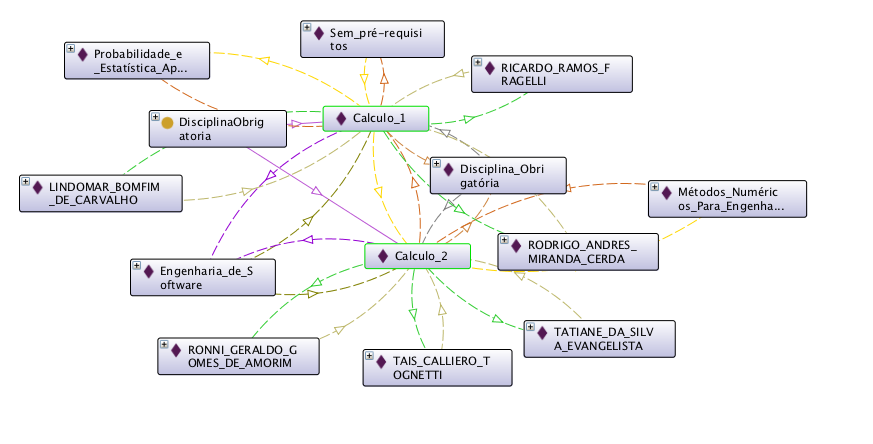
\includegraphics[width=0.9\textwidth]{imagens/ontologia}
	\caption{Exemplo da Ontologia}
	\label{img:ontologia}
\end{figure}

\subsection{Hierarquia de Classes} % (fold)
\label{sub:hierarquia_de_classes}

	Antes da criação da ontologia, efetuou-se uma modelagem conceitual para identificar quais seriam as possíveis entidades que representariam o domínio. Brainstorms e demais exercícios, como a construção de arquivos XML para representar o contexto, ajudaram na definição preliminar de quais classes seriam necessárias.
	
	O segundo passo foi, com a definição preliminar das entidades em mãos, definir a hierarquia de classes. Isto é, como tais classes e suas variações se organizam do ponto de vista da classificação de elementos. Por enquanto, ainda não há representação das propriedades das classes, ou de relações entre instâncias de diferentes entidades.

\begin{figure}[H]
	\centering
	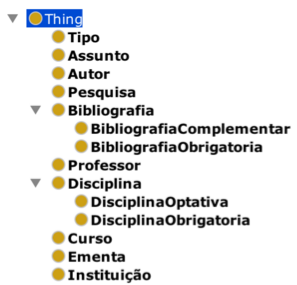
\includegraphics[width=0.5\textwidth]{imagens/hierarquia}
	\caption{Exemplo da Hierarquia de Classes}
	\label{img:hierarquia}
\end{figure}

\begin{figure}[H]
	\centering
	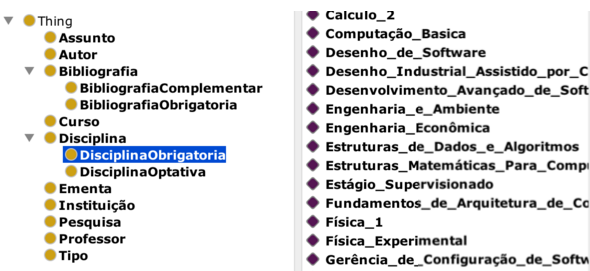
\includegraphics[width=0.7\textwidth]{imagens/hierarquia2}
	\caption{Hierarquia de Classes}
	\label{img:hierarquia2}
\end{figure}

\begin{figure}[H]
	\centering
	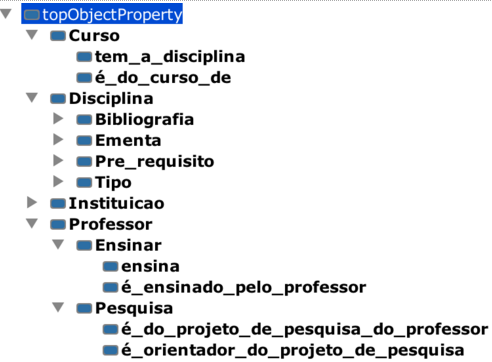
\includegraphics[width=0.5\textwidth]{imagens/hierarquia3}
	\caption{Hierarquia de Classes}
	\label{img:hierarquia3}
\end{figure}

 A hierarquia de classes deve ser feita com cuidado, e deve representar o contexto de maneira consistente, visto que é o elemento de maior importância para que os motores de inferência realizem classificações. Por exemplo, na ontologia realizada, disciplinas obrigatórias são logicamente disjuntas de disciplinas optativas. As propriedades de atributos e objetos, e as características lógicas de cada um destes elementos serão feitos com base nesta árvore de classes.

% subsection hierarquia_de_classes (end)

\subsection{Instâncias e Propriedades} % (fold)
\label{sub:inst_ncias_e_propriedades}

As instâncias das entidades serão criadas de acordo com a estrutura de classes definidas, e serão a representação de fato dos elementos do mundo real na base de dados de conhecimento. Por exemplo, cada curso, disciplina, e professor serão instâncias das respectivas classes na base de dados construida.

\begin{figure}[H]
	\centering
	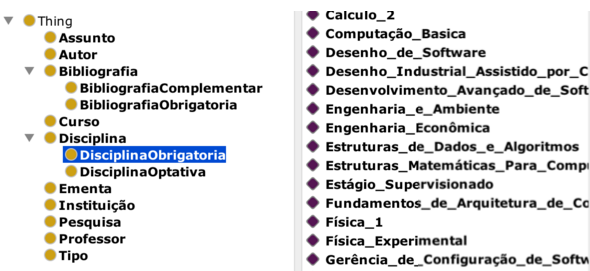
\includegraphics[width=0.7\textwidth]{imagens/hierarquia2}
	\caption{Hierarquia de Classes}
	\label{img:hierarquia4}
\end{figure}

Cada uma destas instâncias possui atributos e relaciona com outras instâncias de outras classes. Por exemplo, uma disciplina específica possui um código, pertence a um curso, e é ministrada por um professor. Para representar tais relações são definidas propriedades de atributos e objetos, que também estarão classificadas por restrições lógicas.
	
	Por exemplo, existem duas propriedades logicamente inversas entre uma disciplina e um professor, "é ensinada por um professor", e "ensina uma disciplina".

% subsection inst_ncias_e_propriedades (end)